\section{Segunda Consigna: Gráficos y Análisis}

Luego de la breve explicación de como se han implementado las herramientas a utilizar, y de haber propuesto 2 rutas a analizar, procedemos a mostrar los resultados obtenidos de las mismas. Para poder realizar los siguientes análisis, lo que hicimos fue: Correr la herramienta \textit{traceroute} a lo largo del dia, cada media hora con un script, durante 12 horas.

\subsection{Rutas encontradas}

Primero, vamos a presentar las rutas encontradas para las IPs propuestas. Se presentaran en formato tabla, y se indicara la ubicación de cada IP segun las herramientas de geolocalización. Las tablas se encuentran en la sección ``Anexo'' de este informe, y se encontraran referenciadas con un link para poder ir directo hacia ellas.

\subsubsection{Universidad de Helsinki (Finlandia)}

El enlace encontrado fue el siguiente:

\begin{itemize}
	\item Entre la IP 195.22.220.92 ubicada en Argentina (Tigre) Segun Geo IP Tool y IP Location, y la IP 149.3.183.11 ubicada en Itala, según las mismas herramientas de geolocalización
\end{itemize}

En el cuadro \ref{table:ruta-finlandia} se muestra como el enlace submarino se debería encontrar entre Argentina y Italia. Esta ruta, fue el resultado de 27 corridas de \textit{traceroute} a lo largo del dia, por lo que es lo mas certero que da nuestra herramienta. En la ruta se ve como al llegar al continente europeo, las IPs van saltando entre IPs locales de Suecia y Finlandia, hasta llegar al host destino.\\

Una cosa a destacar, es la aparición de varios $\Delta$RTT negativos, incluso habiendo promediado los RTT de 10 paquetes distintos, y que ademas como se puede ver, todos fueron exitosos, y solo hubo 1 cambio de IP al inicio del \textit{traceroute}, en donde luego de 8 intentos cambio la IP. Esto muestra como por mas de que se promedien varios RTT, la cercanía de estos nodos, hacen que los RTT varíen mucho. Para eso esta bueno también tener el valor del desvió standard de los intentos, asi tenemos una aproximación de entre que valores puede estar verdaderamente el RTT, con alta probabilidad.

\subsubsection{Universidad de Oxford (Inglaterra)}

Para esta IP, el posible enlace encontrado es el siguiente:

\begin{itemize}
	\item Entre la IP 4.68.111.121 ubicada en Estados Unidos (Chicago) Segun Geo IP Tool y IP Location, y la IP 212.187.139.166 ubicada en Inglaterra (Londres) según las mismas herramientas
\end{itemize}

El resultado de esta ruta se encuentra en el cuadro \ref{table:ruta-inglaterra} A diferencia de la la ruta vista en el punto anterior, esta resulto tener algunas particularidades. Para empezar, el enlace que tiene el mayor $\Delta$RTT, tiene ambos extremos en Estados Unidos, uno en Virginia y el otro en Kansas (según Geo IP Tool y IP Location). Por otro lado, hay otro salto grande que se observa, que es entre el hop 7 y 9, y aquí si ambos extremos están en distintos continentes. Nunca conseguimos que el hop 8 responda el paquete ping, ya que muy probablemente sea un router que descarta los paquetes de tipo ICMP. Esto es un comportamiento bastante habitual que tiene algunos routers.

De todas maneras, según se ve, el enlace debe estar entre Estados Unidos e Inglaterra. Probando también para otras IPs aledañas a la utilizada, obtuvimos los mismo resultados, por lo que optamos por igual quedarnos con esta.

\subsection{Test de Grubbs}

En los resultados que mostramos anteriormente, se vio el $\Delta$RTT del enlace submarino para una sola corrida del \textit{traceroute}, pero esto fue solo para dar un primer vistaso y una primera estimación sobre donde podría encontrarse el enlace submarino. Lo que ahora queremos mostrar, es el resultado que dio el Test de Grubbs, sobre los enlaces anteriormente encontrados, y ver si efectivamente son outliers, y potenciales enlaces submarinos. Recordar que para que el test indique el valor es un outlier o no, se debe cumplir que el estadístico del test G, sea mayor que la condición de rechazo C\\

ACLARACIÓN: Si bien las tablas no es un buen método para presentar datos, en esta ocasión decidimos si utilizarla, ya que se pueden ver todos los valores para todas las corridas del test de Grubbs. Estos son, el p-valor del \textit{normaltest} (herramienta de Python para verificar si una distribucion es normal o no), el estadístico G y el valor para la condición de rechazo C. \\

\subsubsection{Universidad de Helsinki (Finlandia)}

Como se puede ver en el cuadro \ref{table:grubbs-finlandia}, el test de grubbs indica que los $\Delta$RTT del enlace visto en el punto anterior (desde 195.22.220.92 a 149.3.183.11), son outliers de la muestra. Esto reafirma el hecho de que aquí se encuentre un enlace submarino. También se ve como en un solo caso, el test indico que no hay outliers en la muestra, y ademas, el $\Delta$RTT mas grande, no es el enlace visto anteriormente. \\

Si se realiza una mirada mas de cerca sobre los resultados de esta ejecución, se podrá ver como tiene varios $\Delta$RTT muy grandes en comparación a otras ejecuciones. De echo esto hace que el \textit{normaltest} indique que es una distribución normal, pero sin embargo, el test de grubbs indica que el máximo valor no es un outlier. Debido a estas inconsistencias con respecto a las demás ejecuciones, se opto por ignorar esta ejecución, y asumir que fue influenciada por el estado de la red particular de ese momento.


\subsubsection{Universidad de Oxford (Inglaterra)}

En este caso, el test de Grubbs dio que el enlace con mayor $\Delta$RTT era un outlier, pero como vimos con las herramientas de geolocalización de IPs, este enlace probablemente no sea un enlace submarino. Debido a esto, optamos por volver a ejecutar el test de Grubbs, pero esta vez quitando este outlier, para tratar de identificar la presencia de un segundo outlier, y así poder ver si según el test, el enlace que nosotros creemos que es el enlace submarino, es también un outlier según el test de Grubbs. Los resultados pueden verse en la tabla \ref{table:grubbs-inglaterra}\\

Según el test, estos enlaces son outliers de la muestra, y reafirma el hecho de que sea un enlace submarino. No hay mucho mas a destacar de este resultado, salvo quizás otro caso donde las IPs resultantes fueron otras, pero al igual que el caso que tuvimos para la ruta de la universidad de Helsinki, decidimos que esto fue debido a una influencia del trafico en la red al momento de realizar la captura.


\subsection{Aumento del RTT a lo largo de la ruta}

Para tener una mejor visibilidad sobre los RTT de los hops de ambas rutas, presentamos un gráfico de lineas en donde se pueden ver 3 distintas corridas  de nuestra herramienta. No incluimos todas las corridas en el gráfico, ya que resultaba poco legible, y ademas prácticamente toda las corridas tuvieron los mismo tiempos RTTs. Estas se pueden ver en los set de datos adjuntos a este informe.

\subsubsection{Universidad de Helsinki (Finlandia)}

En el gráfico de la figura \ref{fig:rtts-finlandia}, se puede ver como los RTT son muy constantes al principio de la ruta, pero luego al llegar al posible enlace submarino según las heramienta de geolocalizacion y el test de grubbs, se ve un salto del RTT muy grande.

\begin{figure}[H]
  \begin{center}
    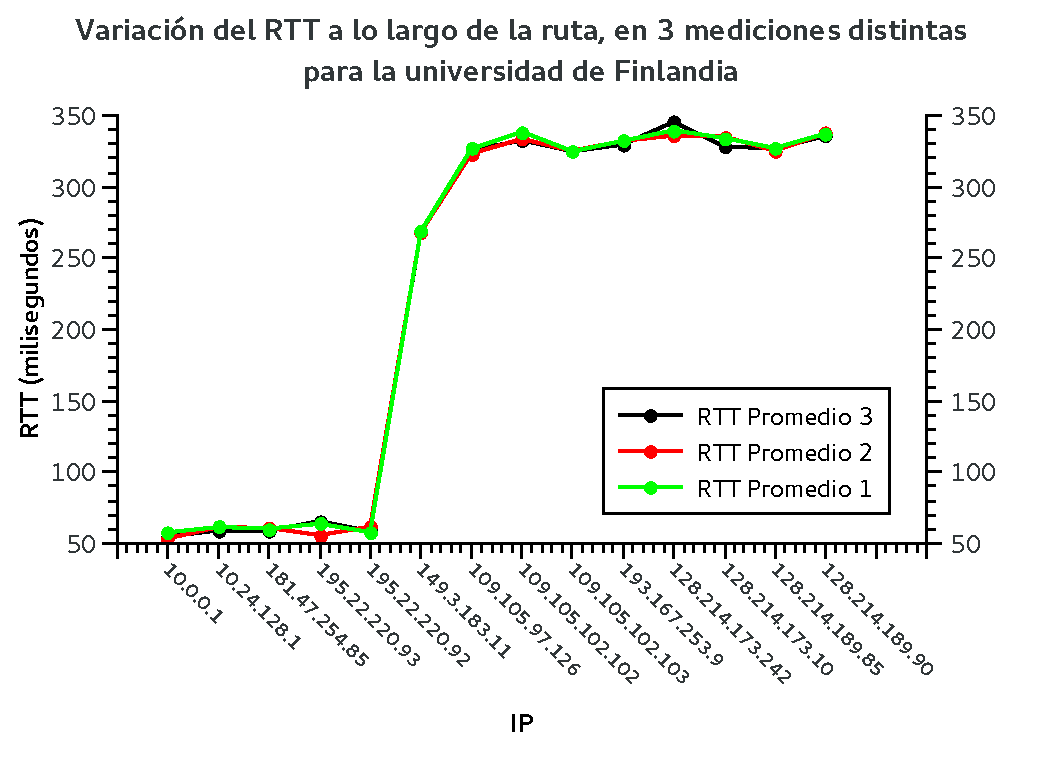
\includegraphics[]{graficos/finlandia-rtts.pdf}
	\caption{Aumento del RTT a lo largo de la ruta de Finlandia}
    \label{fig:rtts-finlandia}  
  \end{center}
\end{figure}

\subsubsection{Universidad de Oxford (Inglaterra)}

En este caso, se puede ver como en realidad tenemos 2 saltos de RTT importantes, los cuales son los analizados anteriormente. Como las herramientas de geolicalizacion de IPs, indican que los extremos del enlace que produce el $\Delta$RTT mas grande, están ambas en Estados Unidos (Entre los estados de Virginia y Kansas), lo que quizá puede estar pasando, es que este tiempo tan alto de RTT se produzca por un encolamiento muy grande en algún router. También existe la posibilidad de que las herramientas de geolocalizacion de IPs tengan información errónea sobre estas IPs.

\begin{figure}[H]
  \begin{center}
    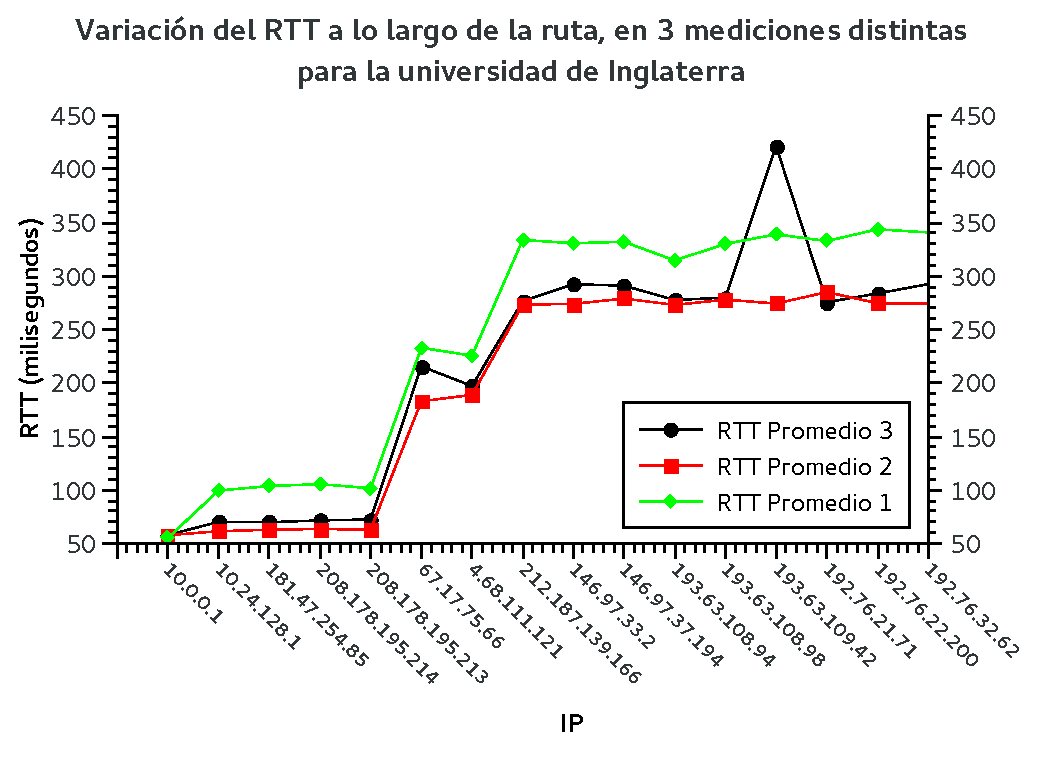
\includegraphics[]{graficos/inglaterra-rtts.pdf}
	\caption{Aumento del RTT a lo largo de la ruta de Inglaterra}
    \label{fig:rtts-inglaterra}  
  \end{center}
\end{figure}

\subsection{Variación del $\Delta$RTT a lo largo del día}

Para realizar el siguiente análisis, se utilizaron las ejecuciones realizadas cada media hora, a lo largo de 12 horas. Reiteramos que estas ejecuciones se encuentran adjuntadas a este informe. La idea es intentar mostrar como varia el RTT de los enlaces, dependiendo del horario, lo cual hace que varíe el trafico de la red. Algo a tener en cuenta sobre estos gráficos, que cada columna NO es en si un solo RTT, ya que nuestra herramienta promedia el RTT de 10 paquetes consecutivos.

\subsubsection{Universidad de Helsinki (Finlandia)}

Como se puede ver en la figura \ref{fig:finlandia-drtt-enlace-dia}, el RTT del enlace varía constantemente, y llega a un pico a las 8 de la madrugada (Hora Argentina). También se puede ver un ligero decrecimiento al entrar en horas de la madrugada, como también un crecimiento pasadas las 7 de la madrugada. Es bastante razonable que esto ocurra ya que, a las 00:00 horas de Argentina, en Italia (Segundo extremo del enlace) son las 04:00 AM, por lo que ambos países deben tener un trafico de red bastante reducido en ese momento.

\begin{figure}[H]
  \begin{center}
    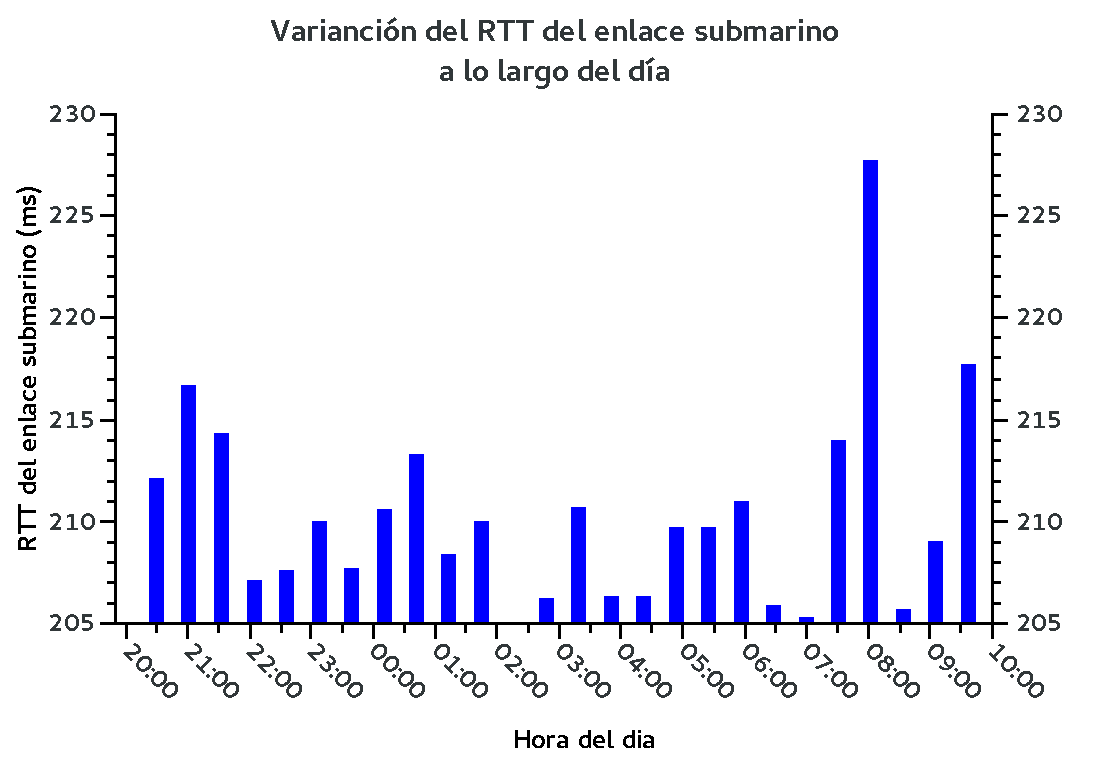
\includegraphics[scale=0.8]{graficos/finlandia-drtt-enlace-dia.pdf}
	\caption{Variacion del  $\Delta$RTT a lo largo del día}
    \label{fig:finlandia-drtt-enlace-dia}  
  \end{center}
\end{figure}

\subsubsection{Universidad de Oxford (Inglaterra)}

Aclaramos que este análisis se hizo sobre el que produjo el segundo mayor $\Delta$RTT, el cual es el que nosotros creemos que es submarino. En el gráfico de la figura \ref{fig:inglaterra-drtt-enlace-dia} se puede ver algo muy parecido a lo que se ve en el gráfico \ref{fig:finlandia-drtt-enlace-dia}. Se ve también como en promedio hay un leve decrecimiento en horas de la madrugada, y un pico muy alto a las 8 AM.

\begin{figure}[H]
  \begin{center}
    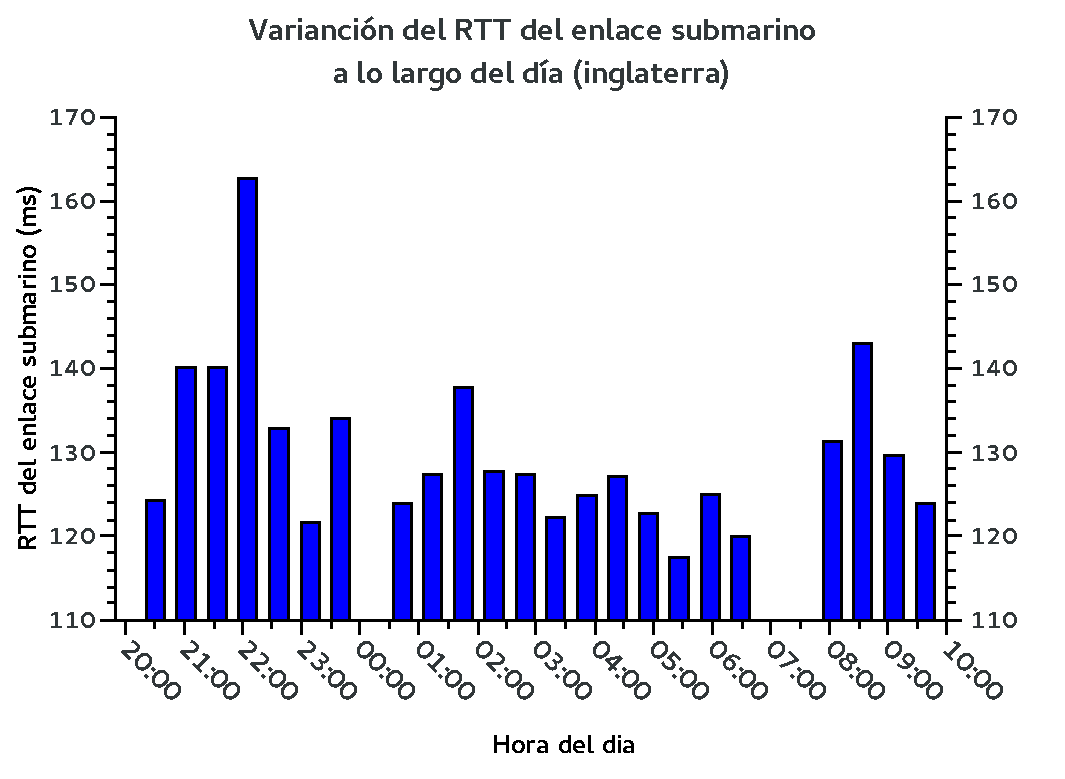
\includegraphics[scale=0.8]{graficos/inglaterra-drtt-enlace-dia.pdf}
	\caption{Variacion del  $\Delta$RTT a lo largo del día}
    \label{fig:inglaterra-drtt-enlace-dia}  
  \end{center}
\end{figure}

\subsection{Mapas de las rutas encontradas (Aproximado)}

En las figuras \ref{fig:mapa-finlandia} y \ref{fig:mapa-inglaterra} se encuentra un mapa aproximado, realizado con la herramienta Google Maps, sobre las rutas que encontramos. De esta manera se puede tener una visión global del camino que pueden tomar los paquetes.

\begin{figure}[H]
  \begin{center}
    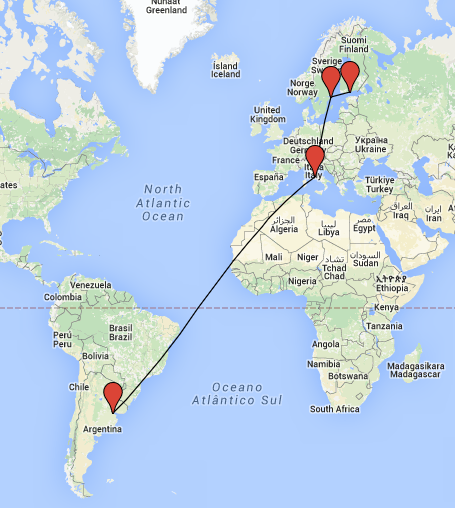
\includegraphics[scale=1]{graficos/finlandia.PNG}
	\caption{Mapa de la ruta a Finlandia}
    \label{fig:mapa-finlandia}  
  \end{center}
\end{figure}

\begin{figure}[H]
  \begin{center}
    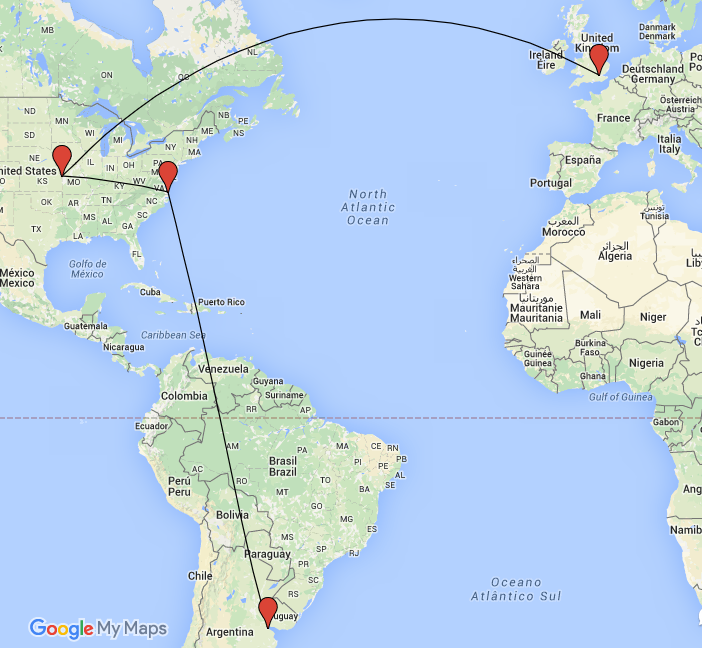
\includegraphics[scale=1]{graficos/inglaterra.PNG}
	\caption{Mapa de la ruta a Inglaterra}
    \label{fig:mapa-inglaterra}  
  \end{center}
\end{figure}